\documentclass[12pt]{report}
\usepackage[utf8]{inputenc}
\usepackage[russian]{babel}
%\usepackage[14pt]{extsizes}
\usepackage{listings}

% Для листинга кода:
\lstset{ %
language=python,                 % выбор языка для подсветки (здесь это С)
basicstyle=\small\sffamily, % размер и начертание шрифта для подсветки кода
numbers=left,               % где поставить нумерацию строк (слева\справа)
numberstyle=\tiny,           % размер шрифта для номеров строк
stepnumber=1,                   % размер шага между двумя номерами строк
numbersep=5pt,                % как далеко отстоят номера строк от подсвечиваемого кода
showspaces=false,            % показывать или нет пробелы специальными отступами
showstringspaces=false,      % показывать или нет пробелы в строках
showtabs=false,             % показывать или нет табуляцию в строках            
tabsize=2,                 % размер табуляции по умолчанию равен 2 пробелам
captionpos=t,              % позиция заголовка вверху [t] или внизу [b] 
breaklines=true,           % автоматически переносить строки (да\нет)
breakatwhitespace=false, % переносить строки только если есть пробел
escapeinside={\#*}{*)}   % если нужно добавить комментарии в коде
}

% Для измененных титулов глав:
\usepackage{titlesec, blindtext, color} % подключаем нужные пакеты
\definecolor{gray75}{gray}{0.75} % определяем цвет
\newcommand{\hsp}{\hspace{20pt}} % длина линии в 20pt
% titleformat определяет стиль
\titleformat{\chapter}[hang]{\Huge\bfseries}{\thechapter\hsp\textcolor{gray75}{|}\hsp}{0pt}{\Huge\bfseries}


% plot
\usepackage{pgfplots}
\usepackage{filecontents}
\usetikzlibrary{datavisualization}
\usetikzlibrary{datavisualization.formats.functions}
\begin{filecontents}{bubble_straight.dat}
100  0.0 
200 0.0101
300 0.01970
400 0.0233
500 0.08998
\end{filecontents}
\begin{filecontents}{insert_straight.dat}
100  0.0 
200 0.0
300 0.0
400 0.0
500 0.0
\end{filecontents}
\begin{filecontents}{quick_straight.dat}
100  0.0 
200 0.0099
300 0.0149
400 0.0350
500 0.0401
\end{filecontents}

\begin{filecontents}{bubble_rev.dat}
100  0.009697
200 0.0101
300 0.02792
400 0.07021
500 0.10028
\end{filecontents}
\begin{filecontents}{insert_rev.dat}
100  0.0 
200 0.0
300 0.01099
400 0.0246
500 0.03731
\end{filecontents}
\begin{filecontents}{quick_rev.dat}
100  0.0 
200 0.01019
300 0.00897
400 0.01993
500 0.03486
\end{filecontents}

\begin{filecontents}{bubble_rand.dat}
100  0.00505
200 0.0300
300 0.04987
400 0.09032
500 0.1666
\end{filecontents}
\begin{filecontents}{insert_rand.dat}
100  0.0 
200 0.00504
300 0.01192
400 0.029708
500 0.044880
\end{filecontents}
\begin{filecontents}{quick_rand.dat}
100  0.0 
200 0.0
300 0.000997
400 0.0
500 0.0030333
\end{filecontents}

\usepackage{graphicx}
\graphicspath{{src/}}
\DeclareGraphicsExtensions{.pdf,.png,.jpg}

\begin{document}
%\def\chaptername{} % убирает "Глава"
\begin{titlepage}
	\centering
	{\scshape\LARGE МГТУ им. Баумана \par}
	\vspace{3cm}
	{\scshape\Large Лабораторная работа №3\par}
	\vspace{0.5cm}	
	{\scshape\Large По курсу: "Анализ алгоритмов"\par}
	\vspace{1.5cm}
	{\huge\bfseries Алгоритмы сортировки\par}
	\vspace{2cm}
	\Large Работу выполнил: Мокеев Даниил, ИУ7-54\par
	\vspace{0.5cm}
	\LargeПреподаватели:  Волкова Л.Л., Строганов Ю.В.\par

	\vfill
	\large \textit {Москва, 2019} \par
\end{titlepage}

\tableofcontents

\newpage
\chapter*{Введение}
\addcontentsline{toc}{chapter}{Введение}

На сегодняшний день существует не одна вариация алгоритмов сортировки. Все они различаются по скорости сортировки и по объему необходимой памяти. 
Цель данной лабораторной работы - обучение расчету трудоемкости алгоритмов

Алгоритмы сортировки часто применяются в практике программирования. В том числе в областях связанных с математикой, физикой, компьютерной графикой и т.д.

\chapter{Аналитическая часть}
\section{Сортировка пузырьком}
Алгоритм состоит из повторяющихся проходов по сортируемому массиву. За каждый проход элементы последовательно сравниваются попарно и, если порядок в паре неверный, выполняется обмен элементов.

\section{Сортировка вставками}
На каждом шаге выбирается один из элементов неотсортированной части массива (максимальный/минимальный) 
и помещается на нужную позицию в отсортированную часть массива. 

\section{Быстрая сортировка}
Общая идея алгоритма состоит в следующем:

\begin{enumerate}
  	\item Выбрать из массива элемент, называемый опорным. Это может быть любой из элементов массива. От выбора опорного элемента не зависит корректность алгоритма, но в отдельных случаях может сильно зависеть его эффективность.
	\item Сравнить все остальные элементы с опорным и переставить их в массиве так, чтобы разбить массив на три непрерывных отрезка, следующих друг за другом: «элементы меньшие опорного», «равные» и «большие».
	\item Для отрезков «меньших» и «больших» значений выполнить рекурсивно ту же последовательность операций, если длина отрезка больше единицы.
\end{enumerate}
На практике массив обычно делят не на три, а на две части: например, «меньшие опорного» и «равные и большие»; такой подход в общем случае эффективнее, так как упрощает алгоритм разделения

\chapter{Конструкторская часть}
\section{Схемы алгоритмов}
В данном разделе будут рассмотрены схемы алгоритмов пузырьком с флагом (\ref{ris:imageSB}), сортировки вставками (\ref{ris:imageIS}), быстрой сортировки (\ref{ris:imageQS}).

\begin{figure}[h]
\center{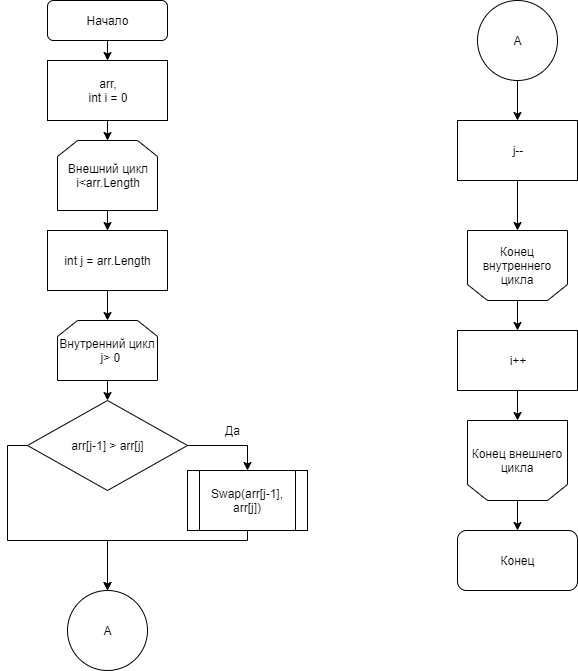
\includegraphics[height = 18cm]{BubbleSort.png}}
\caption{Схема алгоритма сортировки пузырьком}
\label{ris:imageSB}
\end{figure}

\newpage
\begin{figure}[h]
\center{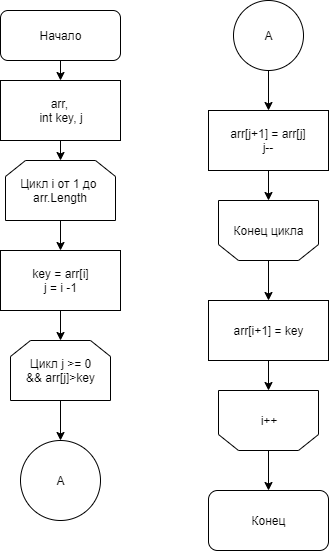
\includegraphics[height = 18cm]{InsertSort.png}}
\caption{Схема алгоритма сортировки вставками}
\label{ris:imageIS}
\end{figure}

\newpage
\begin{figure}[h]
\center{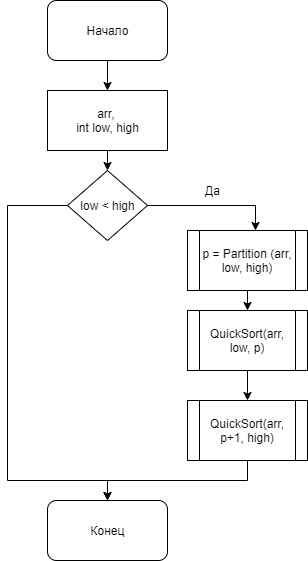
\includegraphics[height = 18cm]{QuickSort.png}}
\caption{Схема алгоритма быстрой сортировки}
\label{ris:imageQS}
\end{figure}

\newpage
\begin{figure}[h]
\center{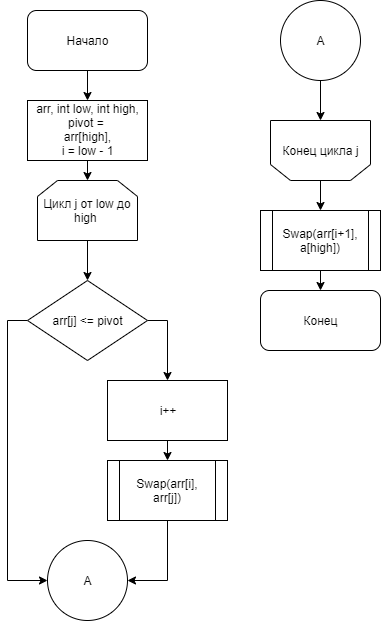
\includegraphics[height = 18cm]{Partition.png}}
\caption{Схема алгоритма Partition}
\label{ris:imageP}
\end{figure}

\section{Трудоемкость алгоритмов}
Введем модель трудоемкости для оценки алгоритмов:
\begin{enumerate}
  	\item  базовые операции стоимостью 1 — +, -, *, /, =, ==, <=, >=, !=, +=, [], ++, -- получение полей класса
	\item оценка трудоемкости цикла: Fц = a + N*(a + Fтела), где a - условие цикла
	\item стоимость условного перехода возьмем за 0, стоимость вычисления условия остаётся.
\end{enumerate}

Далее будет приведены оценки трудоемкости алгоритмов. Построчная оценка трудоемкости сортировки пузырькм с флагом (Табл. 2.1).

\subsection{Сортировка вставками}
\begin{center}
Табл. 2.1 Построчная оценка веса
	\begin{tabular}{|l c|} 
 	\hline
	Код & Вес \\ [0.5ex] 
 	\hline
 	for i in range(1, len(a)): & 1+n*2\\
 	\hline
	key = a[i] & 2\\
	\hline
	j = i-1 & 2\\
	\hline
	while (j >= 0 and a[j] > key): & n*4\\
	\hline
	a[j+1] = a[j] & 4\\
	\hline
	\j -= 1 & 1\\
	\hline
	a[j+1] = key & 3\\
	\hline
	\end{tabular}
\end{center}

\hspace*{5mm}
\textbf{Лучший случай:} отсортированный массив. При этом все внутренние циклы состоят всего из одной итерации.\newline
Трудоемкость: $T(n) = 1 + 2n * (2+2+3)  =  2n * 7 = 14n + 1 = O(n)$

\textbf{Худший случай:} массив отсортирован в обратном нужному порядке. Каждый новый элемент сравнивается со всеми в отсортированной последовательности.
Все внутренние циклы будут состоять из j итераций. \newline
Трудоемкость: $T(n) = 1+n*(2+2+4n*(4+1)+3) = 2n*n+7n+1 =  O(n^{2})$

 \subsection{Сортировка пузырьком}
\textbf{Лучший случай:} Массив отсортирован; не произошло ни одного обмена за 1 проход -> выходим из цикла \newline
Трудоемкость:  $1+2n*(1 + 2n*4) = 1+2n+16n*n=  O(n^{2})$

\textbf{Худший случай:}  Массив отсортирован в обратном порядке; в каждом случае происходил обмен\newline
Трудоемкость: $1+2n*(1 + 2n*(4+5)) = O(n^2)$

\subsection{Быстрая сортировка}
\hspace*{5mm}
\textbf{Лучший случай:} сбалансированное дерево вызовов$^{[2]}$ \(O(n*log(n))\)  
В наиболее благоприятном случае процедура PARTITION приводит к двум подзадачам, размер каждой из которых не превышает $\frac{n}{2}$, поскольку размер одной из них равен $\frac{n}{2}$ , а второй$\frac{n}{2} - 1$. В такой ситуации быстрая сортировка работает намного производительнее, и время ее работы описывается следующим рекуррентным соотношением: $T(n) = 2T(\frac{n}{2}) + O(n)$,где мы не обращаем внимания на неточность, связанную с игнорированием функций “пол” и “потолок”, и вычитанием 1. Это рекуррентное соотношение имеет решение ; $T(n) =O(nlgn)$. При сбалансированности двух частей разбиения на каждом уровне рекурсии мы получаем асимптотически более быстрый алгоритм.

Фактически любое разбиение, характеризующееся конечной константой пропорциональности, приводит к образованию дерева рекурсии высотой $O(lgn)$ со стоимостью каждого уровня, равной $O(n)$. Следовательно, прилюбой постоянной пропорции разбиения полное время работы быстрой сортировки составляет $O(nlgn)$.

\textbf{Худший случай:} несбалансированное дерево $^{[2]}$ $O(n^2)$
Поскольку рекурсивный вызов процедуры разбиения, на вход которой подается массив размером 0, приводит к немедленному возврату из этой процедуры без выполнения каких-ли-бо операций, $T(0) = O(1)$. Таким образом, рекуррентное соотношение, описывающее время работы процедуры в указанном случае, записывается следующим образом: 
$T(n) =T(n-1) +T(0) + O(n) =T(n-1) + O(n)$. Интуитивно понятно, что при суммировании промежутков времени, затрачиваемых на каждый уровень рекурсии, получается арифметическая прогрессия, что приводит к результату $O(n^2)$.

\section{Вывод}
Сортировка пузырьком: лучший - $O(n)$, худший - $O(n^2)$ \newline
Сортировка вставками: лучший - $O(n)$, худший - $O(n^2)$ \newline
Быстрая сортировка: лучший - $O(nlgn)$, худший - $O(n^2)$ \newline

\chapter{Технологическая часть}
\section{Выбор ЯП}
Я выбрал в качестве Python языком программирования, потому как он достаточно удобен и гибок.

Время работы алгоритмов было замерено с помощью функции time() из библиотеки time.

\section{Описание структуры ПО}
Ниже представлена IDEF0 диаграмма (\ref{ris:imageIDEF}), описывающая структуру программы.
\begin{figure}[h]
\center{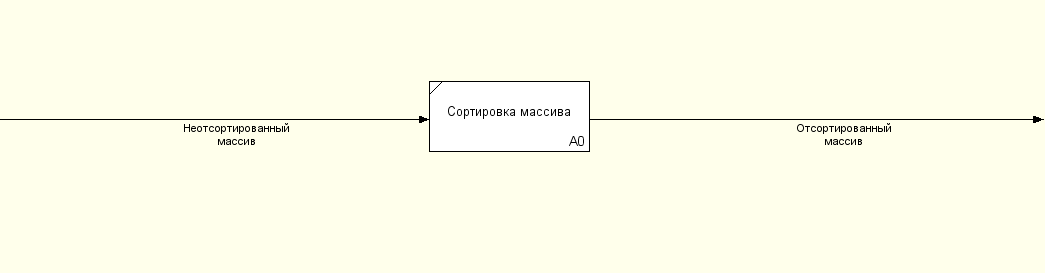
\includegraphics[scale=0.35]{idf.png}} 
\caption{Функциональная схема сортировки массива (IDEF0 диаграмма 1 уровня)}
\label{ris:imageIDEF}
\end{figure}

\section{Сведения о модулях программы}
Программа состоит из:
\begin{itemize}
	\item lab03.py - файл, в котором находятся функции сортировки
\end{itemize}

\begin{lstlisting}[label=some-code,caption=Сортировка пузырьком]
def bubbleSort(a):
    for i in range(len(a)):
        for j in range(len(a)-1, 0, -1):
            if a[j-1] > a[j]:
                a[j-1], a[j] = a[j], a[j-1]

    return a
\end{lstlisting}

\begin{lstlisting}[label=some-code,caption=Сортировка вставками]
def insertSort(a):
    for i in range(1, len(a)):
        key = a[i]
        j = i-1
        while (j >= 0 and a[j] > key):
            a[j+1] = a[j]
            j -= 1
        a[j+1] = key
    return a
\end{lstlisting}

\begin{lstlisting}[label=some-code,caption=Быстрая сортировка]
def quickSort(a, low, high):
    if low < high:
        pi = partition(a, low, high)
        quickSort(a, low,pi)
        quickSort(a, pi+1, high)
    return a
\end{lstlisting}

\begin{lstlisting}[label=some-code,caption=Partition]
def partition(a,low, high):
    i = low - 1
    pivot = a[high]
    for j in range(low, high):
        if a[j] <= pivot:
            i += 1
            a[i], a[j] = a[j], a[i]
    a[i+1],a[high] = a[high], a[i+1]
    return (i+1)
\end{lstlisting}

\chapter{Исследовательская часть}

Был проведен замер времени работы каждой из сортировок.
\section{Примеры работы}
\begin{figure}[h]
\center{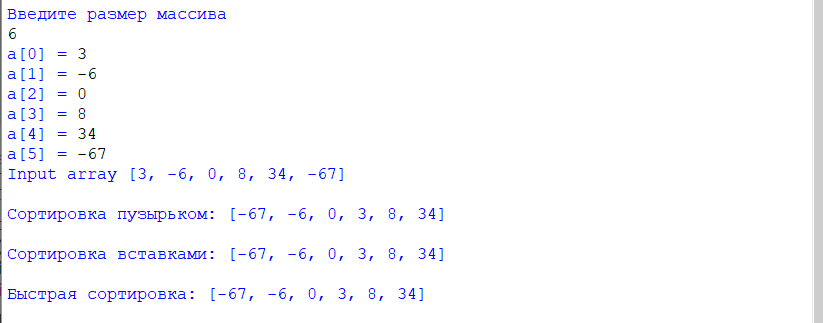
\includegraphics[scale=1.35]{show.png}} 
\caption{Пример работы программы}
\label{ris:example}
\end{figure}
\section{Постановка эксперемента}
Будем измерять время работы алгоритмов на отсортированных, отсортированных в обратном порядке и случайно сгенерированных массивах. Для замера времени будем использовать функцию time.
\subsection{Сортировка пузырьком}
\begin{center}
	\begin{tabular}{|c c c c|} 
 	\hline
	len & Отсортированный, сек. & Обратный порядок, сек. & Случайный,сек \\ [0.5ex] 
 	\hline\hline
 	100 & 0.0 & 0.00969 & 0.00505 \\
 	\hline
 	200 & 0.0101 & 0.0101 & 0.03002\\
 	\hline
	300 & 0.01970 & 0.02792 & 0.04987 \\
	\hline
	400 & 0.0233 & 0.07021 & 0.09032 \\
	\hline
	500 & 0.08998 & 0.10028 & 0.16667\\
	\hline
	\end{tabular}
\end{center}
\subsection{Сортировка вставками}
\begin{center}
	\begin{tabular}{|c c c c|} 
 	\hline
	len & Отсортированный, сек. & Обратный порядок, сек. & Случайный,сек \\ [0.5ex] 
 	\hline\hline
 	100 & 0.0 & 0.0 & 0.0 \\
 	\hline
 	200 & 0.0 & 0.0 & 0.0050\\
 	\hline
	300 & 0.0 & 0.010990 & 0.01192 \\
	\hline
	400 & 0.0 & 0.0246 & 0.0297\\
	\hline
	500 & 0.0 & 0.03731 & 0.044881\\
	\hline
	\end{tabular}
\end{center}

\subsection{Быстрая сортировка}
\begin{center}
	\begin{tabular}{|c c c c|} 
 	\hline
	len & Отсортированный, сек. & Обратный порядок, сек. & Случайный,сек \\ [0.5ex] 
 	\hline\hline
 	100 & 0.0 & 0.0 & 0.0 \\
 	\hline
 	200 & 0.00991 & 0.01019 & 0.0\\
 	\hline
	300 & 0.0149 & 0.00897 & 0.00099 \\
	\hline
	400 & 0.0350 & 0.01993 & 0.0\\
	\hline
	500 & 0.04014 & 0.03486 & 0.00303\\
	\hline
	\end{tabular}
\end{center}


\begin{figure}
\begin{tikzpicture}
\begin{axis}[
    	axis lines = left,
    	xlabel = $len$,
    	ylabel = {$time$},
	legend pos=north west,
	ymajorgrids=true
]
\addplot[color=red] table[x index=0, y index=1] {bubble_straight.dat}; 
\addplot[color=green] table[x index=0, y index=1] {insert_straight.dat};
\addplot[color=blue, mark=square] table[x index=0, y index=1] {quick_straight.dat};

\addlegendentry{bubble}
\addlegendentry{insert}
\addlegendentry{quick}
\end{axis}
\end{tikzpicture}
\caption{Сравнение сортировки уже отсортированных массивов} \label{plot:straight}
\end{figure}
\par
\begin{figure}
    \centering
\begin{tikzpicture}
\begin{axis}[
    	axis lines = left,
    	xlabel = $len$,
    	ylabel = {$time$},
	legend pos=north west,
	ymajorgrids=true
]
\addplot[color=red] table[x index=0, y index=1] {bubble_rev.dat}; 
\addplot[color=green] table[x index=0, y index=1] {insert_rev.dat};
\addplot[color=blue, mark=square] table[x index=0, y index=1] {quick_rev.dat};

\addlegendentry{bubble}
\addlegendentry{insert}
\addlegendentry{quick}
\end{axis}
\end{tikzpicture}
\caption{Сравнение сортировки массивов, отсортированных в обратном порядке} \label{plot:rev}
\end{figure}
\par
\begin{figure}
\begin{tikzpicture}
\begin{axis}[
    	axis lines = left,
    	xlabel = $len$,
    	ylabel = {$time$},
	legend pos=north west,
	ymajorgrids=true
]
\addplot[color=red] table[x index=0, y index=1] {bubble_rand.dat}; 
\addplot[color=green] table[x index=0, y index=1] {insert_rand.dat};
\addplot[color=blue, mark=square] table[x index=0, y index=1] {quick_rand.dat};

\addlegendentry{bubble}
\addlegendentry{insert}
\addlegendentry{quick}
\end{axis}
\end{tikzpicture}
\caption{Сравнение сортировки случайных массивов} \label{plot:rand}
\end{figure}
\newpage
\subsection{Заключение эксперементальной части}
Были протестированы алгоритмы сортировки на массивах размерами 100…500 с шагом 100. Рассмотрены отсортированные, отсортированные в обратном порядке массивы и массивы со случайными значениями.

В результате тестирования было получено, что лучшее время сортировки показывают на отсортированных массивах. Худшие значения сортировки показывают на обратно отсортированных массивах, причём чем больше размер такого массива, тем медленнее работают сортировки. 

При сравнении времени работы алгоритмов можно сделать вывод, что на размерах массива до 300 элементов время работы алгоритмов приближено к 0 сек. При работе с массивами больших размеров сортировка пузырьком показывает наихудший результат. При сортировки случайных массивов лучшее время показывает быстрая сортировка.

\chapter*{Заключение}
\addcontentsline{toc}{chapter}{Заключение}
В ходе выполнения данной лабораторной работы были реализованы три алгоритма сортировки: сортировка пузырьком, сортировка вставками и быстрая сортировка. Был проведён анализ каждого алгоритма и измерено время работы алгоритмов для массивов разных размеров. Была оценена трудоёмкость алгоритмов.

Лучшее время работы все сортировки показывают на отсортированных массивах: при обработке массива в 500 элементов сортировка пузырьком - 0.005 сек, вставками и быстрая сортировка – 0.0 сек. Худшее время алгоритмы сортировки показали при работе с массивами, отсортированными в обратном порядке. Причём чем больше размерность такого массива, тем медленнее работает алгоритм.

Был сделан вывод, что на массивах размерностью до 300 элементов время работы всех трёх алгоритмов близится к 0 сек. При обработке массивов больших размеров, например, 500, лучший результат показала быстрая сортировка, худшее – сортировка пузырьком.


\chapter*{Список литературы}
\addcontentsline{toc}{chapter}{Список литературы}
\begin{enumerate}
    \item  Кормен, Т., Лейзерсон, Ч., Ривест, Р., Штайн, К. Глава 7. Быстрая сортировка // Алгоритмы: построение и анализ = Introduction to Algorithms / Под ред. И. В. Красикова. — 2-е изд. — М.: Вильямс, 2005.
    \item Левитин А. В. Глава 4. Метод декомпозиции: Быстрая сортировка // Алгоритмы. Введение в разработку и анализ — М.: Вильямс, 2006. 
\end{enumerate}

\end{document}

